\documentclass[letterpaper]{article}
\usepackage[margin=1in]{geometry}
\usepackage[utf8]{inputenc}
\usepackage{textcomp}
\usepackage{amssymb}
\usepackage{natbib}
\usepackage{graphicx}
\usepackage{gensymb}
\usepackage{amsthm, amsmath, mathtools}
\usepackage[dvipsnames]{xcolor}
\usepackage{enumerate}
\usepackage{mdframed}
\usepackage[most]{tcolorbox}
\usepackage{csquotes}
% https://tex.stackexchange.com/questions/13506/how-to-continue-the-framed-text-box-on-multiple-pages

\tcbuselibrary{theorems}

\newcommand{\R}{\mathbb{R}}
\newcommand{\Z}{\mathbb{Z}}
\newcommand{\N}{\mathbb{N}}
\newcommand{\Q}{\mathbb{Q}}
\newcommand{\C}{\mathbb{C}}
\newcommand{\code}[1]{\texttt{#1}}
\newcommand{\mdiamond}{$\diamondsuit$}
\newcommand{\PowerSet}{\mathcal{P}}
\newcommand{\Mod}[1]{\ (\mathrm{mod}\ #1)}
\DeclareMathOperator{\lcm}{lcm}

%\newtheorem*{theorem}{Theorem}
%\newtheorem*{definition}{Definition}
%\newtheorem*{corollary}{Corollary}
%\newtheorem*{lemma}{Lemma}
\newtheorem*{proposition}{Proposition}


\newtcbtheorem[number within=section]{theorem}{Theorem}
{colback=green!5,colframe=green!35!black,fonttitle=\bfseries}{th}

\newtcbtheorem[number within=section]{definition}{Definition}
{colback=blue!5,colframe=blue!35!black,fonttitle=\bfseries}{def}

\newtcbtheorem[number within=section]{corollary}{Corollary}
{colback=yellow!5,colframe=yellow!35!black,fonttitle=\bfseries}{cor}

\newtcbtheorem[number within=section]{lemma}{Lemma}
{colback=red!5,colframe=red!35!black,fonttitle=\bfseries}{lem}

\newtcbtheorem[number within=section]{example}{Example}
{colback=white!5,colframe=white!35!black,fonttitle=\bfseries}{def}

\newtcbtheorem[number within=section]{note}{Important Note}{
        enhanced,
        sharp corners,
        attach boxed title to top left={
            xshift=-1mm,
            yshift=-5mm,
            yshifttext=-1mm
        },
        top=1.5em,
        colback=white,
        colframe=black,
        fonttitle=\bfseries,
        boxed title style={
            sharp corners,
            size=small,
            colback=red!75!black,
            colframe=red!75!black,
        } 
    }{impnote}
\usepackage[utf8]{inputenc}
\usepackage[english]{babel}
\usepackage{fancyhdr}
\usepackage[hidelinks]{hyperref}

\pagestyle{fancy}
\fancyhf{}
\rhead{MATH 180A}
\chead{Friday, April 15, 2022}
\lhead{Lecture 8}
\rfoot{\thepage}

\setlength{\parindent}{0pt}

\begin{document}

\section{Conditional Probability: Discrete Case}
Let $A$ be an event. Recall that $\PR(A)$ is the probability that $A$ occurs. Now, suppose that we're given some additional information. Then, this information may not completely determine whether $A$ has occurred, but it might give us some valuable partial information. 

\begin{mdframed}[]
    (Example.) Suppose that a magician rolls a fair die. Let $A$ be the event that we roll a 6. Then, we know that 
    \[\PR(A) = \frac{1}{6}.\]
    Now, let's suppose that the magician tells you that the result is an even number (either 2, 4, or 6), but does not yet reveal the full result of the roll to you. How does the probability of $A$ change? It's certainly not $\frac{1}{6}$ since we know that it has to be an even number. Intuitively, the answer is $\frac{1}{3}$; this is particularly because the die originally was uniform, so there is no reason why -- when the magician got an even number -- the even numbers have a heavier weight. 
\end{mdframed}

\subsection{What is Conditional Probaiblity?}
Conditional probability is the study of probability under the presence of partial information. 
\begin{definition}{Conditional Probability}{}
    Let $A$ and $B$ be two events such that 
    \begin{itemize}
        \item $A$ is  the event of interest.
        \item $B$ is the event that encodes the partial information that we have. 
    \end{itemize}
    Suppose that $\PR(B) > 0$. Then, the \textbf{conditional probability} of $A$, given that $B$ has occurred, is denoted by $\PR(A | B)$.  
\end{definition}
\textbf{Remarks:} 
\begin{itemize}
    \item We require $\PR(B) > 0$; if $\PR(B) = 0$, then this would imply that $B$ would never occur anyways. 
    \item All of the given information is on the \emph{right} of the bar. 
\end{itemize}
In our example above, $A$ would be the event of interest and $B$ is the event coming from the magician telling us that the roll was an even number. 

\subsection{Finding Conditional Probability}
How do we find $\PR(A | B)$? 
\begin{mdframed}[]
    (Example, Continued.) In the previous example, it's clear that the probability of rolling a 6 should change from $\frac{1}{6}$ to $\frac{1}{3}$ once we found out that the roll is an even number. Additionally, the roll is uniformly random -- now, we know that there is one of \emph{three} possible numbers, so it should still remain uniformly random, but just on the sample space $\{2, 4, 6\}$ instead of the original sample space $\{1, 2, 3, 4, 5, 6\}$. 

    \bigskip 

    So, if $A$ is the event that we rolled a 6, and $B$ is the even that we rolled an even number, notice that: 
    \begin{itemize}
        \item $\PR(A) = \frac{1}{6}$: This is the probability that we roll a 6.
        \item $\PR(B) = \frac{1}{2}$: This is the probability that we will any even number.
        \item $\PR(A \cap B) = \frac{1}{6}$: This is the probability that both events occur. Notice that $A$ is a subset of $B$; therefore, $A \cap B = A$. 
    \end{itemize}
    Intuitively, we expect $\PR(A | B) = \frac{1}{3}$, and indeed we note that 
    \[\frac{\PR(A \cap B)}{\PR(B)} = \frac{1 / 6}{1 / 2} = \frac{1}{3}.\]
\end{mdframed}
In general, it is true that 
\[\boxed{\PR(A | B) = \frac{\PR(A \cap B)}{\PR(B)}}.\]
Why is this true? 
\begin{mdframed}[]
    (Informal Discussion.) Suppose that the sample space is $\Omega$ and we have two events $A, B \subset \Omega$. Then, consider the following Venn Diagram, where $\PR(A)$ is represented by $\frac{\text{area}(A)}{\text{area}(\Omega)}$ and $\PR(B)$ is represented by $\frac{\text{area}(B)}{\text{area}(\Omega)}$. 
    \begin{center}
        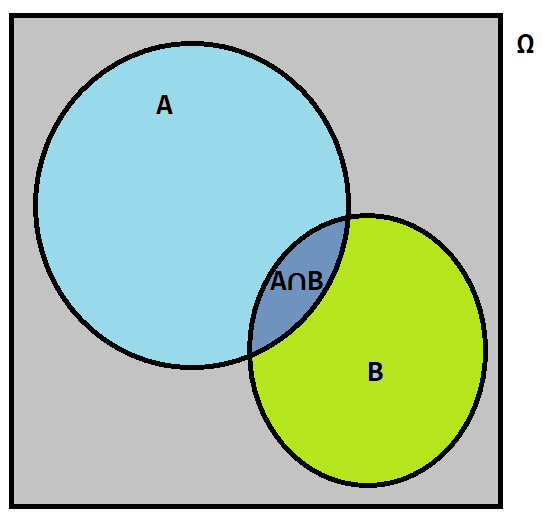
\includegraphics[scale=0.7]{../assets/venn1.png}
    \end{center}
    Now, the idea is that when we randomly throw a dart at the ``dartboard'' $\Omega$, it will ``land in'' $A$ with probability $\PR(A)$ and similarly for $B$. 
    
    \bigskip 
    
    Now, suppose that we are told that the dart landed somewhere in $B$, but we don't know anything else beyond that. Then, since the dart was thrown randomly, it should be in some random position in $B$ (i.e. nowhere in $B$ should be more likely than anywhere else). Now, what is the probability that it landed in $A$, \emph{given} that it landed somewhere in $B$?
    \begin{center}
        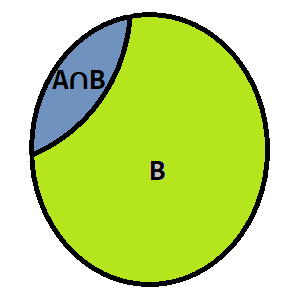
\includegraphics[scale=0.7]{../assets/venn2.png}
    \end{center}
    The answer is to find out what is the probability that the dart landed in the intersection, that is, in the $A \cap B$ region. In this case, we can consider their \emph{ratios} -- in this case, we consider the area of $A \cap B$ against the area of $B$. Then, in effect, $B$ becomes the new sample space (i.e. the ``dartboard''), since we now know that the outcome of the experiment is in $B$. Therefore, we have 
    \[\PR(A | B) = \frac{\PR(A \cap B)}{\PR(B)}.\]
\end{mdframed}
With this in mind, we can now give a formal definition.
\begin{definition}{Conditional Probability}{}
    Let $A$ and $B$ be two events. Suppose that $\PR(B) > 0$. Then, the \textbf{conditional probability} of $A$, given that $B$ has occurred, is $\PR(A | B) = \frac{\PR(A \cap B)}{\PR(B)}$.  
\end{definition}
Recall that $\PR(\omega)$ is a probability distribution on the sample space $\Omega$ \emph{if} we have 
\begin{itemize}
    \item $\PR(\omega) \geq 0$ for all $\omega \in \Omega$, and 
    \item $\sum_{\omega \in \Omega} \PR(\omega) = 1$. 
\end{itemize}
Note that the function $\PR(\omega | B)$ is \emph{also} a probability distribution, but now the \emph{sample space} is $B$. In particular:
\begin{enumerate}
    \item $\PR(\omega | B) = \frac{\PR(\omega \cap B)}{\PR(B)} = \frac{\PR(\omega)}{\PR(B)} \geq 0$ for all $\omega \in B$. Note that this is true since $\PR(B) > 0$ and $\PR(\omega) \geq 0$ for all $\omega \in \Omega$. 
    \item $\sum_{\omega \in B} \PR(\omega | B) = \frac{1}{\PR(B)} \sum_{\omega \in B} \PR(\omega) = \frac{1}{\PR(B)} \PR(B) = 1$. 
\end{enumerate}
Note that, by multiplying both sides of the conditional probability formula $P(A | B)$ by $P(B)$, we get the following formula:
\begin{theorem}{Probability Chain Rule}{}
    \[\PR(A \cap B) = \PR(B) \PR(A | B).\]
\end{theorem}
\textbf{Remarks:}
\begin{itemize}
    \item The conditional probability formula only holds when $\PR(B) > 0$. 
    \item The probability chain rule $\PR(A \cap B) = \PR(B) \PR(A | B)$ holds even when $\PR(B) = 0$. 
\end{itemize}

\begin{mdframed}[nobreak=true]
    (Example.) On sunny days, Vito goes for a walk with probability $\frac{4}{5}$. On rainy days, Vito goes for a walk with probability $\frac{1}{10}$. Suppose that, in San Diego, it rains on any given day with probability $3\%$. Find the probability that Vito goes for a walk today. 

    \begin{mdframed}[]
        We let $W$ be the event that Vito goes for a walk today; we want to find $\PR(W)$. Let $S$ be the event that it is sunny today.

        \bigskip 

        We know that it rains with a $3\%$ chance, so the change of it being sunny is $97\%$, or $\frac{97}{100}$. Thus, $\PR(S) = \frac{97}{100}$. We also know that the probability that Vito goes for a walk, \emph{given} that it is sunny\footnote{Note that we were not told that the probability of him going for a walk \emph{and} it being sunny is $\frac{4}{5}$; all we're told is that \emph{if} it is a sunny day, then he'll go for a walk with probability $\frac{4}{5}$.}, is $\PR(W | S) = \frac{4}{5}$. Likewise, the probability that Vito goes for a walk, given that it is rainy (not a sunny day), is $\PR(W | S^C) = \frac{1}{10}$. 

        \bigskip 

        Recall that, by the Law of Total Probability, we have 
        \[\PR(W) = \PR(W \cap S) + \PR(W \cap S^C) \implies \PR(W \cap S) = \PR(W) - \PR(W \cap S^C).\]
        Additionally, we know that 
        \[\PR(W \cap S^C) = \PR(S^C) \PR(W | S^C) = \frac{3}{100} \frac{1}{10} = \frac{3}{1000}.\]
        Therefore, applying this formula to the probability chain rule and solving, we get the following work: 
        \begin{equation*}
            \begin{aligned}
                \PR(W \cap S) &= \PR(S) \PR(W | S) && \text{Probability Chain Rule}\\ 
                    &\implies \PR(W) - \PR(W \cap S^C) = \PR(S) \PR(W | S) && \text{Applying Law of Total Probability} \\ 
                    &\implies \PR(W) = \PR(S) \PR(W | S) + \PR(W \cap S^C) && \text{Add } \PR(W \cap S^C) \text{ to Both Sides}\\ 
                    &\implies \PR(W) = \frac{97}{100} \frac{4}{5} + \frac{3}{1000} && \text{Substitute Values} \\ 
                    &\implies \PR(W) = \frac{779}{1000} && \text{Simplify}
            \end{aligned}
        \end{equation*}
    \end{mdframed}
\end{mdframed}

\subsection{Law of Total Probability, Conditional Version}
Recall that, if $A \subset \Omega$ is an event, and if $B_1, \dots, B_n$ are partitions of $\Omega$, then, the Law of Total Probability is given by  
\[\PR(A) = \sum_{i = 1}^{n} \PR(A \cap B_i).\]
Using the probability chain rule, we have
\[\PR(A) = \sum_{i = 1}^{n} \PR(B_i) \PR(A | B_i).\]
This is the conditional version of the Law of Total Probability.
\begin{theorem}{Law of Total Probability, Conditional Version}{}
    Suppose that $A \subset \Omega$ is an event and that the events $B_1, \dots, B_n$ partition that sample space $\Omega$. Then, we have that 
    \[\PR(A) = \sum_{i = 1}^{n} \PR(B_i) \PR(A | B_i).\]
\end{theorem}

\subsection{Independent Events}
Now that we have defined conditional probability, we can formally define what it means for events to be independent. 
\begin{definition}{Independent Events}{}
    Two events $A, B$ are \textbf{independent} if either 
    \begin{enumerate}
        \item $\PR(A) = 0$, 
        \item $\PR(B) = 0$, or 
        \item $\PR(A | B) = \PR(A)$ and $\PR(B | A) = \PR(B)$, in the case that both $\PR(A) > 0$ and $\PR(B) > 0$.
    \end{enumerate}
\end{definition}
\textbf{Remark:} With regards to (3), the occurrence of $B$ does not affect the occurrence of $A$, and vice versa. 

\bigskip 

Now, by the probability chain rule, if two events $A$ and $B$ are independent, then 
\[\PR(A \cap B) = \PR(A) \PR(B).\]
Indeed, $\PR(A \cap B) = \PR(A | B) \PR(B) = \PR(A) \PR(B)$. This introduces the next theorem: 
\begin{theorem}{}{}
    If $A$ and $B$ are independent, then 
    \[\PR(A \cap B) = \PR(A) \PR(B).\]
\end{theorem}

Now, independence is more complicated when more than two events are involved. In particular:
\begin{definition}{}{}
    Events $A_1, \dots, A_n$ are \textbf{mutually independent} if, for any $A_{i_1}, \dots, A_{i_k}$, we have that 
    \[\PR\left(\bigcap_{i = 1}^{k} A_{i_k} \right) = \prod_{i = 1}^{k} \PR(A_{i_k}).\]
\end{definition}
In particular, we have
\[\PR\left(\bigcap_{i = 1}^{n} A_{i} \right) = \prod_{i = 1}^{n} \PR(A_{i}).\]
A weaker version onf independence is as follows: 
\begin{definition}{}{}
    Events $A_1, \dots, A_n$ are \textbf{pairwise independent} if each pair $A_i$, $A_j$ (with $i \neq j$) are independent.
\end{definition}
Note that if $n > 2$, then mutually and pairwise independence are \textbf{not} equivalent.

\subsection{Joint Probability Distributions}
Suppose that $X_1, \dots, X_n$ are discrete random variables with PMFs 
\[p_{X_i} = \PR(X_i = x).\]
Then, the joint PMF of the RV $\mathbf{X} = (X_1, \dots, X_n)$ is the function 
\[p_{\mathbf{X}}(x_1, \dots, x_n) = \PR(X_1 = x_1, \dots, X_n = x_n)\]
for all $x_1, \dots, x_n$. Here, we can think of this as a function from a sample space to $\R^n$ (higher dimensions).

\bigskip 

Often, it can be quite difficult to find the joint PMFs. However, in the special case that $X_1, \dots, X_n$ are \textbf{independent}, it is just the product of the individual PMFs; that is, 
\[p_{\mathbf{X}}(x_1, \dots, x_n) = \prod_{i = 1}^{n} p_{X_i}(x_i).\]
We say that $X_1, \dots, X_n$ are \textbf{independent and identically distributed}\footnote{This is known as \textbf{independent trial process} in the textbook.} (IID for short) if they are mutually independent, and all have the same distribution. An example of this is a sequence $X_1, \dots, X_n$ of $n$ Bernoulli($p$) trials. In this case, each trial has the simple distribution 
\[\PR(X_i = 1) = p\]
and 
\[\PR(X_i = 0) = 1 - p.\]
In general, though, in such a process, $X_i$ can have any given distribution. In any case, if $X_1, \dots, X_n$ are IIDs, then their joint PMF takes the simple form known as a \textbf{product distribution}. In particular, since the $X_i$'s are IIDs, they have the same PMFs $p(x) = \PR(X_i) = x$ no matter what $i$ is. Hence, the joint PMF is just 
\[\PR(X_1 = x_1, \dots, X_n = x_n) = \prod_{i = 1}^{n} p(x_i).\]
For example, in a sequence of Bernoulli($p$) trials, 
\[\PR(X_1 = x_1, \dots, X_n = x_n) = p^k (1 - p)^{n - k},\]
if exactly $k$ of the $x_i = 1$ and the other $n - k$ of the $x_i = 0$. 

\end{document}